\documentclass[12pt]{article}

\usepackage{amsmath, mathtools}
\usepackage{amsfonts}
\usepackage{amssymb}
\usepackage{graphicx}
\usepackage{colortbl}
\usepackage{xr}
\usepackage{hyperref}
\usepackage{longtable}
\usepackage{xfrac}
\usepackage{tabularx}
\usepackage{float}
\usepackage{siunitx}
\usepackage{booktabs}
\usepackage{caption}
\usepackage{pdflscape}
\usepackage{afterpage}
\usepackage[usenames,dvipsnames,svgnames,table]{xcolor}
\usepackage{txfonts}

\usepackage[round]{natbib}

%\usepackage{refcheck}

\hypersetup{
    bookmarks=true,         % show bookmarks bar?
      colorlinks=true,       % false: boxed links; true: colored links
    linkcolor=Purple,          % color of internal links (change box color with 
    %linkbordercolor)
    citecolor=ForestGreen,        % color of links to bibliography
    filecolor=WildStrawberry,      % color of file links
    urlcolor=Cerulean           % color of external links
}

%% Comments

\usepackage{color}

\newif\ifcomments\commentstrue

\ifcomments
\newcommand{\authornote}[3]{\textcolor{#1}{[#3 ---#2]}}
\newcommand{\todo}[1]{\textcolor{red}{[TODO: #1]}}
\else
\newcommand{\authornote}[3]{}
\newcommand{\todo}[1]{}
\fi

\newcommand{\wss}[1]{\authornote{blue}{SS}{#1}}
\newcommand{\an}[1]{\authornote{magenta}{Author}{#1}}

% For easy change of table widths
\newcommand{\colZwidth}{1.0\textwidth}
\newcommand{\colAwidth}{0.13\textwidth}
\newcommand{\colBwidth}{0.82\textwidth}
\newcommand{\colCwidth}{0.1\textwidth}
\newcommand{\colDwidth}{0.05\textwidth}
\newcommand{\colEwidth}{0.8\textwidth}
\newcommand{\colFwidth}{0.17\textwidth}
\newcommand{\colGwidth}{0.5\textwidth}
\newcommand{\colHwidth}{0.28\textwidth}

% Used so that cross-references have a meaningful prefix
\newcounter{defnum} %Definition Number
\newcommand{\dthedefnum}{GD\thedefnum}
\newcommand{\dref}[1]{GD\ref{#1}}
\newcounter{datadefnum} %Datadefinition Number
\newcommand{\ddthedatadefnum}{DD\thedatadefnum}
\newcommand{\ddref}[1]{DD\ref{#1}}
\newcounter{theorynum} %Theory Number
\newcommand{\tthetheorynum}{T\thetheorynum}
\newcommand{\tref}[1]{T\ref{#1}}
\newcounter{tablenum} %Table Number
\newcommand{\tbthetablenum}{T\thetablenum}
\newcommand{\tbref}[1]{TB\ref{#1}}
\newcounter{assumpnum} %Assumption Number
\newcommand{\atheassumpnum}{P\theassumpnum}
\newcommand{\aref}[1]{A\ref{#1}}
\newcounter{goalnum} %Goal Number
\newcommand{\gthegoalnum}{P\thegoalnum}
\newcommand{\gsref}[1]{GS\ref{#1}}
\newcounter{instnum} %Instance Number
\newcommand{\itheinstnum}{IM\theinstnum}
\newcommand{\iref}[1]{IM\ref{#1}}
\newcounter{reqnum} %Requirement Number
\newcommand{\rthereqnum}{P\thereqnum}
\newcommand{\rref}[1]{R\ref{#1}}
\newcounter{lcnum} %Likely change number
\newcommand{\lthelcnum}{LC\thelcnum}
\newcommand{\lcref}[1]{LC\ref{#1}}

\newcommand{\progname}{Companion Cube Calculator} % PUT YOUR PROGRAM NAME HERE
\newcommand{\prognameAbbrv}{$C^{3}$}

\usepackage{fullpage}

\begin{document}

\title{Companion Cube Calculator} 
\author{Geneva Smith}
\date{\today}
	
\maketitle

\pagenumbering{roman}
\tableofcontents

\begin{table}[bp]
\caption{\bf Revision History}
\begin{tabularx}{\textwidth}{p{3cm}p{2cm}X}
\toprule {\bf Date} & {\bf Version} & {\bf Notes}\\
\midrule
September 26, 2017 & 1.1 & Completed the first draft of the General System 
Description (Section \ref{general})\\
September 25, 2017 & 1.0 & Completed the first draft of the Introduction 
(Section \ref{intro})\\
\bottomrule
\end{tabularx}
\end{table}

\newpage
\section{Reference Material}

This section records information for easy reference.

\subsection{Table of Units}

The tasks performed by the \prognameAbbrv{} tool are unitless.

\subsection{Table of Symbols}

The table that follows summarizes the symbols used in this document along with
their units.  The choice of symbols was made to be consistent with the heat
transfer literature and with existing documentation for solar water heating
systems.  The symbols are listed in alphabetical order.

\renewcommand{\arraystretch}{1.2}
%\noindent \begin{tabularx}{1.0\textwidth}{l l X}
\noindent \begin{longtable*}{l l p{12cm}} \toprule
\textbf{Symbol} & \textbf{Unit} & \textbf{Description}\\
\midrule 
$b^x$ & - & Base number $b$ raised to the power of variable $x$\\
$D(x)$ & - & Domain of $x$\\
$f(X)$ & - & A function of a variable set $X$\\
$R(f(X))$ & - & Range of $f(X)$\\
$\varmathbb{R}$ & - & The set of real numbers\\
$x^n$ & - & Variable $x$ raised to the power of constant $n$ \\
\bottomrule
\end{longtable*}

\subsection{Abbreviations and Acronyms}

\renewcommand{\arraystretch}{1.2}
\begin{tabular}{l l} 
  \toprule		
  \textbf{Text} & \textbf{Description}\\
  \midrule 
  A & Assumption\\
  CRPG & Computer Role-Playing Game\\
  DD & Data Definition\\
  GD & General Definition\\
  GS & Goal Statement\\
  GUI & Graphical User Interface\\
  IM & Instance Model\\
  LC & Likely Change\\
  NPC & Non-Player Character\\
  PS & Physical System Description\\
  R & Requirement\\
  SRS & Software Requirements Specification\\
  \prognameAbbrv{} & \progname{}\\
  T & Theoretical Model\\
  \bottomrule
\end{tabular}

\newpage
\pagenumbering{arabic}

\section{Introduction}
\label{intro}
This document is an SRS for the \progname{} (\prognameAbbrv{}), a mathematical 
tool which determines the range of a user-specified function given the domains 
of the function's variables. This tool is being developed to aid in the 
specification and refinement of GLaDOS, an emotion engine for Non-Player 
Characters (NPCs) in Computer Role-Playing Games (CRPG) as described by 
\citet{glados}.

\subsection{Purpose of Document}
This document outlines the requirements identified for the development of the 
\prognameAbbrv{} tool, including the product goals, product scope, and the 
mathematical models driving the design. It also describes the mathematical 
assumptions, theories, and models used to create the tool. The purpose of 
documenting this information is to aid in future use, maintenance, and 
development of the \prognameAbbrv{} tool.

This document is intended for two reader types -- those who wish to use the 
tool and those who wish to expand the tool. Even though the \progname{} was 
created to aid in the development of a specific system (GLaDOS), the tested 
functions do not have any specific units. This means that it can be used for 
any function that exists in the domain of real numbers ($\varmathbb{R}$). 
Therefore, this document can be used by a user who wishes to use the 
\prognameAbbrv{} tool to determine the range of a specified mathematical 
function. Since the initial development of the \prognameAbbrv{} tool will be 
limited to arithmetic operators, this document includes information that will 
be useful to a developer looking to expand the abilities of the 
\prognameAbbrv{} with additional mathematical models such as trigonometry to 
suit their project.

\subsection{Scope of Requirements} 
The \progname{} calculates the mathematical range of a user-defined function 
using the defined variable domains for that function. In the cases where a 
variable domain is not provided, it will be assumed that the range is 
$(-\infty, \infty)$. For the initial version of this product, the mathematical 
operations allowed in an function will be limited to the four arithmetic 
operators ($+$, $-$, $\times$, $\div$, exponents). Future iterations can expand 
this list to include trigonometric functions ($\sin$, $\cos$, $\tan$, $\arcsin$,
$\arccos$, $\arctan$), partial functions, and other useful operations and 
functions.

The purpose of this product is to aid in the design and tuning of the GLaDOS 
architecture, a specialized game engine enables game designers to create 
Non-Player Characters (NPCs) that react to their environment by using models of 
emotion from psychology. One module in the architecture converts information 
from the environment into an internal representation that directs an NPC's 
decision-making. This task requires the specification of numerical functions 
with multiple variables which must be normalized to a range of $[-1,1]$. In 
order to normalize the engine's calculation, the range of the function must be 
known. Currently, the encoded functions are not well-informed by observation or 
scientific research and must be subjected to an iterative process in order to 
address this problem. An automated method of calculating the range of a 
proposed function will make this process faster and less error-prone.

Although this product is being designed for a specific project, the concepts 
involved can be used in similar projects because it does not contain any 
project-specific concepts or models.

\subsection{Characteristics of Intended Reader}
\label{intro_reader}
The intended reader of this document must understand elementary algebra, 
especially interval arithmetic, in the domain of real numbers 
($\varmathbb{R}$). They must also have an understanding of domain and range 
with respect to a function in order to understand the outputs of the product 
and how it relates to its 
inputs.

\subsection{Organization of Document}
This document begins by describing the general description of the \progname{} 
tool (Section \ref{general}), which includes the system context, constraints, 
and the intended users' characteristics. This is followed by a description of 
the problem to be solved, including the models and assumptions that are used to 
solve it (Section \ref{specific}). This description is followed by the 
functional and non-functional requirements of the \prognameAbbrv{} tool 
(Section \ref{requirements}) and the potential changes that will be made to 
them in future iterations (Section \ref{changes}). The last section in this 
document, traceability matrices and graphs, visually describes the dependencies 
between different document components (Section \ref{trace}). This information 
should be used by making changes to the decisions made for this version of the 
tool.

\section{General System Description}
\label{general}

This section identifies the interfaces between the system and its environment,
describes the user characteristics and lists the system constraints.

\subsection{System Context}
The \progname{} tool is a stand-alone application for calculating the range of 
a user-provided function given the known domains of the function's component 
variables. Therefore it is independent and self-contained with respect to 
external organizations, products, and technologies.

The user interface of the \prognameAbbrv{} tool facilitates communication 
between the product and the user, and must contain the ability to exchange user 
inputs and system outputs. In general, the user is responsible for ensuring 
that they have provided a semantically correct function and that their inputs 
do not contain mathematical operations that are not implemented in the tool. 
The \progname{} is responsible for providing an information exchange interface 
between itself and the user, performing mathematical calculations, and 
detecting syntactic errors in the system inputs.

\begin{itemize}
	\item User Responsibilities:
	\begin{itemize}
		\item Provide an function from the domain of real numbers 
		($\varmathbb{R}$) that only contains mathematical operations that are 
		recognized by the system
		\item Provide the mathematical domains of the function's variables if 
		they are known
		\item Ensure that the function given to the tool does not contain 
		semantic errors
		\item Ensure that the products outputs are semantically correct with 
		respect to the target application
	\end{itemize}
	\item \progname{} Responsibilities:
	\begin{itemize}
		\item Allow the user to enter their function and known variable domains 
		as system inputs
		\item For variables with unknown domains, provide default values to be 
		used in calculations
		\item Detect data type mismatch, such as a string of characters instead 
		of a floating point number
		\item Detect bracket mismatches
		\item Calculate and output the mathematical range corresponding to the 
		user's inputs; if a result cannot be calculated, communicate this to 
		the user
	\end{itemize}
\end{itemize}

\subsection{User Characteristics} \label{SecUserCharacteristics}
The end user of \progname{} is also the intended reader (Section 
\ref{intro_reader}) of this document.

\subsection{System Constraints}
The use of a Graphical User Interface (GUI) is useful for the \prognameAbbrv{} 
tool because it can help the user visualize their function during design time 
and debugging. This has implications on the types of languages that this tool 
will be developed in and target platform choices. If a GUI is included in the 
\prognameAbbrv{} design, only Windows platforms will be supported in the 
initial release.

\section{Specific System Description}
\label{specific}
This section first presents the problem description, which gives a high-level
view of the motivation behind the \progname{}. This is followed by the solution 
characteristics specification, presenting the assumptions, theories, 
definitions, and instance models, which are grounded in interval arithmetic. 

\subsection{Problem Description} \label{Sec_pd}
The GLaDOS architecture is a specialized game engine that enables game 
designers to create Non-Player Characters (NPCs) that react to their 
environment by using models of emotion from psychology. A key component of the 
architecture is the primary appraisal module, where inputs from the environment 
are converted into emotion values. The functions currently used for this task 
are not well informed by any scientific research, and will be incrementally 
revised as more information is collected. These new functions are required to 
conform to the same mathematical range as the currently implemented functions. 
Ensuring that this requirement is maintained over consecutive iterations of the 
functions will become tedious and time consuming, distracting from the main 
task of developing more rigorous and explainable emotion functions.

The \progname{} is a tool for calculating the range of a mathematical function 
based on its input variables, which will help make the function design process 
faster and less error-prone when compared to doing it by hand.

\subsubsection{Terminology and  Definitions}

This subsection provides a list of terms that are used in the subsequent
sections and their meaning, with the purpose of reducing ambiguity and making it
easier to correctly understand the requirements:

\begin{itemize}

\item Closed interval: A bounded set that includes its end points; this is 
expressed $[a,b]$
\item Closed interval method: A mathematical method for determining the local 
maximum and minimum values of a function $f(x)$ using a closed domain interval 
$[a,b]$
\item Connected set: a set of values that does not contain any disjoint members
\item Domain ($D(x)$): the set of values for a variable $x$ that are valid in 
$f(X)$
\item Extended real interval: the set of all real numbers that also contains 
$\pm \infty$
\item Open interval: A bounded set of values that does not contain its end 
points; this is expressed $(a,b)$
\item Range ($R(f(X))$): the set of values that are produced by a function 
$f(X)$ with a set of input variables $X$
\item Real interval: a closed, connected set of real numbers

\end{itemize}

\subsubsection{Physical System Description}

The \progname{} tool does not have a physical system component because it 
exists independently of the context of $f(X)$. 

\subsubsection{Goal Statements}

\noindent Given an function and a set of variables, the goal statements are:

\begin{itemize}

\item[GS\refstepcounter{goalnum}\thegoalnum \label{G_range}:] 
Calculate $R(f(X))$.

%\item[GS\refstepcounter{goalnum}\thegoalnum \label{G_unknownDomain}:] 
%Determine $D(x)$ for any $x \in X$ if it is not part of the input set.

\end{itemize}

\subsection{Solution Characteristics Specification}
The instance models that govern \progname{} are presented in
Subsection~\ref{sec_instance}. The information to understand the meaning of the
instance models and their derivation is also presented, so that the instance
models can be verified.

\subsubsection{Assumptions}
This section simplifies the original problem and helps in developing the
theoretical model by filling in the missing information for the physical
system. The numbers given in the square brackets refer to the theoretical model
[T], general definition [GD], data definition [DD], instance model [IM], or
likely change [LC], in which the respective assumption is used.

\begin{itemize}

\item[A\refstepcounter{assumpnum}\theassumpnum \label{A_domain}:] $D(x)$ is a 
closed, real interval. 

\item[A\refstepcounter{assumpnum}\theassumpnum \label{A_interval}:] $R(f(X))$ 
is a closed, real interval.

\item[A\refstepcounter{assumpnum}\theassumpnum \label{A_operators}:] The 
mathematical operators used in $f(X)$ can be found in the set $\{+, -, 
\times, \div, b^x, x^n \}$.

\end{itemize}

\subsubsection{Theoretical Models}\label{sec_theoretical}

This section focuses on the general equations and laws from interval arithmetic 
that the \progname{} is based on. The models presented here are for real 
intervals, which can be constrained to closed, real intervals using 
\ddref{DD_interval} to satisfy \aref{A_domain} and \aref{A_interval}. 
Additional models exist for interval arithmetic, but only the models named in 
\aref{A_operators} are mentioned.

~\newline

\noindent
\begin{minipage}{\textwidth}
\renewcommand*{\arraystretch}{1.5}
\begin{tabular}{| p{\colAwidth} | p{\colBwidth}|}
  \hline
  \rowcolor[gray]{0.9}
  Number& T\refstepcounter{theorynum}\thetheorynum \label{T_addition}\\
  \hline
  Label&\bf Addition on Real Intervals\\
  \hline
  Equation&  $X + Y = \{x + y | x \in X \wedge y \in Y\}$\\
  \hline
  Description & The summation interval of two real intervals $X$ and 
  $Y$ is equal to the set of sums for each pairwise element $x$ and $y$.\\
  \hline
  Source & \citet{intervalarithmetic}\\
  \hline
  Ref.\ By & \iref{I_addition}\\
  \hline
\end{tabular}
\end{minipage}\\

~\newline

\noindent
\begin{minipage}{\textwidth}
	\renewcommand*{\arraystretch}{1.5}
	\begin{tabular}{| p{\colAwidth} | p{\colBwidth}|}
		\hline
		\rowcolor[gray]{0.9}
		Number& T\refstepcounter{theorynum}\thetheorynum \label{T_subtraction}\\
		\hline
		Label&\bf Subtraction on Real Intervals\\
		\hline
		Equation&  $X - Y = \{x - y | x \in X \wedge y \in Y\}$\\
		\hline
		Description & The difference interval of two real intervals $X$ 
		and $Y$ is equal to the set of differences for each pairwise element 
		$x$ and 
		$y$.\\
		\hline
		Source & \citet{intervalarithmetic}\\
		\hline
		Ref.\ By & \iref{I_subtraction}\\
		\hline
	\end{tabular}
\end{minipage}\\

~\newline

\noindent
\begin{minipage}{\textwidth}
	\renewcommand*{\arraystretch}{1.5}
	\begin{tabular}{| p{\colAwidth} | p{\colBwidth}|}
		\hline
		\rowcolor[gray]{0.9}
		Number& T\refstepcounter{theorynum}\thetheorynum 
		\label{T_multiplication}\\
		\hline
		Label&\bf Multiplication on Real Intervals\\
		\hline
		Equation&  $X \times Y = \{x \times y | x \in X \wedge y \in Y\}$\\
		\hline
		Description & The product interval of two real intervals $X$ 
		and $Y$ is equal to the set of products for each pairwise element $x$ 
		and $y$.\\
		\hline
		Source & \citet{intervalarithmetic}\\
		\hline
		Ref.\ By & \iref{I_multiplication}\\
		\hline
	\end{tabular}
\end{minipage}\\

~\newline

\noindent
\begin{minipage}{\textwidth}
	\renewcommand*{\arraystretch}{1.5}
	\begin{tabular}{| p{\colAwidth} | p{\colBwidth}|}
		\hline
		\rowcolor[gray]{0.9}
		Number& T\refstepcounter{theorynum}\thetheorynum 
		\label{T_division}\\
		\hline
		Label&\bf Division on Real Intervals\\
		\hline
		Equation&  $X \div Y = \{z | \exists x \in X, y \in Y \wedge y \neq 0, 
		z = x \div y\}$\\
		\hline
		Description & The quotient interval of two real intervals $X$ and $Y$ 
		is equal to the set of quotients for each pairwise element $x$ and $y$ 
		where $y \neq 0$. If $0 \in Y$, the quotient is not a real interval 
		which contradicts \aref{A_interval}.\\
		\hline
		Source & \citet{intervalarithmetic}\\
		\hline
		Ref.\ By & \iref{I_positivedivision}, \iref{I_negativedivision}\\
		\hline
	\end{tabular}
\end{minipage}\\

~\newline

\noindent
\begin{minipage}{\textwidth}
	\renewcommand*{\arraystretch}{1.5}
	\begin{tabular}{| p{\colAwidth} | p{\colBwidth}|}
		\hline
		\rowcolor[gray]{0.9}
		Number& T\refstepcounter{theorynum}\thetheorynum 
		\label{T_exponents}\\
		\hline
		Label&\bf Real Interval Exponents on a Constant Base Number\\
		\hline
		Equation&  $b^X = \{b^x | x \in X \wedge b > 1\}$\\
		\hline
		Description & The product interval of a constant number $b$ raised to 
		the power of a real interval $X$ is equal to the set of products $b^x$ 
		for 
		each interval element $x$.\\
		\hline
		Source & \url{https://en.wikipedia.org/wiki/Interval_arithmetic}\\
		\hline
		Ref.\ By & \ddref{DD_base}, \iref{I_exponents}\\
		\hline
	\end{tabular}
\end{minipage}\\

~\newline

\noindent
\begin{minipage}{\textwidth}
	\renewcommand*{\arraystretch}{1.5}
	\begin{tabular}{| p{\colAwidth} | p{\colBwidth}|}
		\hline
		\rowcolor[gray]{0.9}
		Number& T\refstepcounter{theorynum}\thetheorynum 
		\label{T_expbase}\\
		\hline
		Label&\bf Constant Exponents on a Real Interval Base 
		Number\\
		\hline
		Equations &  $X^n = \begin{cases}
			\{x^n | x \in X \wedge n 
			\in \varmathbb{N}\} & \text{n is odd}\\
			\{[x_{1}^n,...,x_{z}^n] | x \in X \wedge n 
			\in \varmathbb{N}\} & \text{n is even}\wedge x_{z} \geq x_{z+1} 
			\wedge x_{1} > 0\\
			\{[x_{z}^n,...,x_{1}^n] | x \in X \wedge n 
			\in \varmathbb{N}\} & \text{n is even} \wedge x_{z} < x_{z+1} 
			\wedge x_{Z} < 0\\
			\{[0,...,max\{x_{1}^n,x_{z}^n\}] | x \in X \wedge n 
			\in \varmathbb{N}\} & \text{ELSE}\\
		\end{cases}$
		\newline
		\\
		\hline
		Description & The product interval of a real interval $X$ 
		raised to the power of a constant, natural number $n$ depends on the 
		properties of $X$ and $n$:
		\begin{itemize}
			\item When $n$ is an odd number, the product interval is equal to 
			the set of products $x^n$ for each element $x$
			\item When $n$ is even, the function is monotonically decreasing, 
			and $x_{1} > 0$, the product interval is equal to the set of 
			products $x^n$ for each element $x$
			\item When $n$ is even, the function is monotonically increasing, 
			and $x_{Z} < 0$, the product interval is equal to the set of 
			products $x^n$ for each element $x$ and ordered in the opposite 
			direction of the original interval $X$
			\item Otherwise, the product interval is bounded by $0$ and the 
			maximum product of the first and last elements in the interval set
		\end{itemize}\\
		\hline
		Source & \url{https://en.wikipedia.org/wiki/Interval_arithmetic}\\
		\hline
		Ref.\ By & \ddref{DD_power}, \iref{I_expbase}\\
		\hline
	\end{tabular}
\end{minipage}\\

~\newline

\subsubsection{General Definitions}\label{sec_gendef}
No additional information is required to build the data definitions. 

\subsubsection{Data Definitions}\label{sec_datadef}

This section collects and defines all the data needed to build the instance
models. No dimensions are required because the tasks performed by \progname{} 
are unitless. These definitions are used to constrain the theoretical models to 
such that thay can be translated into instance models on closed, real intervals 
to satisfy \aref{A_domain} and \aref{A_interval}.

~\newline

\noindent
\begin{minipage}{\textwidth}
\renewcommand*{\arraystretch}{1.5}
\begin{tabular}{| p{\colAwidth} | p{\colBwidth}|}
\hline
\rowcolor[gray]{0.9}
Number& DD\refstepcounter{datadefnum}\thedatadefnum \label{DD_interval}\\
\hline
Label& \bf Representation of a Closed, Real Interval\\
\hline
Symbol &$[x, y]$\\
\hline
% Units& $Mt^{-3}$\\
% \hline
  SI Units & -\\
  \hline
  Equation& -\\
  \hline
  Description & The definition $[x,y]$ represents a closed, real interval 
  (\aref{A_domain}, \aref{A_interval}) with endpoints $x$ and $y$.
  \\
  \hline
  Sources& - \\
  \hline
  Ref.\ By & \iref{I_addition}, \iref{I_subtraction}, \iref{I_multiplication}, 
  \iref{I_positivedivision}, \iref{I_negativedivision}, \iref{I_exponents}, 
  \iref{I_expbase}\\
  \hline
\end{tabular}
\end{minipage}\\

~\newline

\noindent
\begin{minipage}{\textwidth}
	\renewcommand*{\arraystretch}{1.5}
	\begin{tabular}{| p{\colAwidth} | p{\colBwidth}|}
		\hline
		\rowcolor[gray]{0.9}
		Number& DD\refstepcounter{datadefnum}\thedatadefnum \label{DD_base}\\
		\hline
		Label& \bf Representation of a Base Number\\
		\hline
		Symbol &$b$\\
		\hline
		% Units& $Mt^{-3}$\\
		% \hline
		SI Units & -\\
		\hline
		Equation& -\\
		\hline
		Description & A constant real number ($\varmathbb{R}$) such that $b > 
		1$
		(\tref{I_exponents}).
		\\
		\hline
		Sources& - \\
		\hline
		Ref.\ By & \iref{I_exponents}\\
		\hline
	\end{tabular}
\end{minipage}\\

~\newline

\noindent
\begin{minipage}{\textwidth}
	\renewcommand*{\arraystretch}{1.5}
	\begin{tabular}{| p{\colAwidth} | p{\colBwidth}|}
		\hline
		\rowcolor[gray]{0.9}
		Number& DD\refstepcounter{datadefnum}\thedatadefnum \label{DD_power}\\
		\hline
		Label& \bf Representation of a Power\\
		\hline
		Symbol &$n$\\
		\hline
		% Units& $Mt^{-3}$\\
		% \hline
		SI Units & -\\
		\hline
		Equation& -\\
		\hline
		Description & A constant natural number ($\varmathbb{N}$)
		(\tref{I_expbase}).
		\\
		\hline
		Sources& - \\
		\hline
		Ref.\ By & \iref{I_expbase}\\
		\hline
	\end{tabular}
\end{minipage}\\

\subsubsection{Instance Models} \label{sec_instance}    

This section transforms the problem defined in Section~\ref{Sec_pd} into 
one which is expressed in mathematical terms. It uses concrete symbols defined 
in Section~\ref{sec_datadef} to replace the abstract symbols in the models 
identified in Sections~\ref{sec_theoretical} and~\ref{sec_gendef}.

The goal \gsref{G_range} is solved by recursively combining instance models 
\iref{I_addition}, \iref{I_subtraction}, \iref{I_multiplication}, 
\iref{I_division}, \iref{I_exponents}, and \iref{I_expbase}. For example, if 
the user provided an equation of the form $a + b \times c$, it is decomposed 
into $a + B$ where $B = b \times c$. This approach is identical to a 
hand-written evaluation except a mechanized approach must explicitly state the 
intermediary steps, which are commonly omitted by humans, in order to complete 
the computational task.

These models can also be used as a specification for the closed interval method 
because of the closed, real interval assumption on $D(x)$ (\aref{A_domain}).

~\newline

\noindent
\begin{minipage}{\textwidth}
\renewcommand*{\arraystretch}{1.5}
\begin{tabular}{| p{\colAwidth} | p{\colBwidth}|}
  \hline
  \rowcolor[gray]{0.9}
  Number& IM\refstepcounter{instnum}\theinstnum \label{I_addition}\\
  \hline
  Label& \bf Addition of closed, real intervals\\
  \hline
  Input&$[x_{1}, y_{1}]$, $[x_{2}, y_{2}]$ from \ddref{DD_interval}\\
  \hline
  Output&$[x_{sum}, y_{sum}]$ such that\\
  &$x_{sum} = x_{1} + x_{2}$, $y_{sum} = y_{1} + y_{2}$,\\
  &$[x_{sum}, y_{sum}]$ is a closed, real interval (\aref{A_interval}) \\
  \hline
  Description&$[x_{1}, y_{1}]$ and $[x_{2}, y_{2}]$ are the domains of two 
  variables in the user's input function $f(X)$.\\
  &The combined boundary values $x_{sum}$ and  $y_{sum}$ are determined 
  using basic arithmetic addition.\\
  & The result, $[x_{sum}, y_{sum}]$, is guaranteed to be a closed, real 
  interval (\aref{A_interval}) due to the closed, real interval constraint on 
  $[x_{1}, y_{1}]$ and $[x_{2}, y_{2}]$ (\aref{A_domain}).
  \\
  \hline
  Sources& ~\cite{intervalarithmetic} \ \\
  \hline
  Ref.\ By & -\\
  \hline
\end{tabular}
\end{minipage}\\

~\newline

\noindent
\begin{minipage}{\textwidth}
	\renewcommand*{\arraystretch}{1.5}
	\begin{tabular}{| p{\colAwidth} | p{\colBwidth}|}
		\hline
		\rowcolor[gray]{0.9}
		Number& IM\refstepcounter{instnum}\theinstnum \label{I_subtraction}\\
		\hline
		Label& \bf Subtraction of closed, real intervals\\
		\hline
		Input&$[x_{1}, y_{1}]$, $[x_{2}, y_{2}]$ from \ddref{DD_interval}\\
		\hline
		Output&$[x_{sub}, y_{sub}]$ such that\\
		&$x_{sub} = x_{1} - x_{2}$, $y_{sub} = y_{1} - y_{2}$,\\
		&$[x_{sub}, y_{sub}]$ is a closed, real interval (\aref{A_interval}) \\
		\hline
		Description&$[x_{1}, y_{1}]$ and $[x_{2}, y_{2}]$ are the domains of 
		two variables in the user's input function $f(X)$. \\
		&The combined boundary values $x_{sub}$ and  $y_{sub}$ are determined 
		using basic arithmetic subtraction.\\
		& The result, $[x_{sub}, y_{sub}]$, is guaranteed to be a closed, real 
		interval (\aref{A_interval}) due to the closed, real interval 
		constraint on $[x_{1}, y_{1}]$ and $[x_{2}, y_{2}]$ (\aref{A_domain}).
		\\
		\hline
		Sources& ~\cite{intervalarithmetic} \ \\
		\hline
		Ref.\ By & -\\
		\hline
	\end{tabular}
\end{minipage}\\

~\newline

\noindent
\begin{minipage}{\textwidth}
	\renewcommand*{\arraystretch}{1.5}
	\begin{tabular}{| p{\colAwidth} | p{\colBwidth}|}
		\hline
		\rowcolor[gray]{0.9}
		Number& IM\refstepcounter{instnum}\theinstnum \label{I_multiplication}\\
		\hline
		Label& \bf Multiplication of closed, real intervals\\
		\hline
		Input&$[x_{1}, y_{1}]$, $[x_{2}, y_{2}]$ from \ddref{DD_interval}\\
		\hline
		Output&$[x_{mul}, y_{mul}]$ such that\\
		&$x_{mul} = \min(M)$, $y_{mul} = \max(M)$, where $M = \{x_{1} \times 
		x_{2}, x_{1} \times y_{2}, y_{1} \times x_{2}, y_{1} \times y_{2}\}$\\
		&$[x_{mul}, y_{mul}]$ is a closed, real interval (\aref{A_interval}) \\
		\hline
		Description&$[x_{1}, y_{1}]$ and $[x_{2}, y_{2}]$ are the domains of 
		two variables in the user's input function $f(X)$. \\
		&The combined boundary value $x_{mul}$ is determined by taking the 
		minimum of all possible products calculated from the sets $[x_{1}, 
		y_{1}]$ and $[x_{2}, y_{2}]$, where $[x_{1}, y_{1}]$ is the 
		multiplier set and $[x_{2}, y_{2}]$ is the multiplicand set\\
		&The combined boundary value $y_{mul}$ is determined by taking the 
		maximum of all possible products calculated from the sets $[x_{1}, 
		y_{1}]$ and $[x_{2}, y_{2}]$, where $[x_{1}, y_{1}]$ is the 
		multiplier set and $[x_{2}, y_{2}]$ is the multiplicand set\\
		& The result, $[x_{mul}, y_{mul}]$, is guaranteed to be a closed, real 
		interval (\aref{A_interval}) due to the closed, real interval 
		constraint on $[x_{1}, y_{1}]$ and $[x_{2}, y_{2}]$ (\aref{A_domain}).
		\\
		\hline
		Sources& ~\cite{intervalarithmetic} \ \\
		\hline
		Ref.\ By & -\\
		\hline
	\end{tabular}
\end{minipage}\\

~\newline

\noindent
\begin{minipage}{\textwidth}
	\renewcommand*{\arraystretch}{1.5}
	\begin{tabular}{| p{\colAwidth} | p{\colBwidth}|}
		\hline
		\rowcolor[gray]{0.9}
		Number& IM\refstepcounter{instnum}\theinstnum 
		\label{I_positivedivision}\\
		\hline
		Label& \bf Division of closed, real intervals (Divisor is a positive 
		interval)\\
		\hline
		Input&$[x_{1}, y_{1}]$, $[x_{2}, y_{2}]$ from \ddref{DD_interval} where 
		$0 \leq x_{2} \leq y_{2}$ and $x_{2} \neq 0$\\
		\hline
		Output&$[x_{div}, y_{div}]$ such that\\
		&\vspace*{-10mm}\begin{center}
			\begin{tabular}{lll}
				$x_{div} = x_{1} \div y_{2}$, & $y_{div} = y_{1} \div x_{2}$ & 
				$0 < x_{1} \leq y_{1}$  \\
				$x_{div} = 0$, & $y_{div} = y_{1} \div x_{2}$ & $x_{1} = 0 
				\wedge x_{1} \leq y_{1}$ \\
				$x_{div} = x_{1} \div x_{2}$, & $y_{div} = y_{1} \div x_{2}$ & 
				$x_{1} < 0 < y_{1}$ \\
				$x_{div} = x_{1} \div x_{2}$, & $y_{div} = 0$ & $y_{1} = 0, 
				x_{1} \leq y_{1}$\\
				$x_{div} = x_{1} \div x_{2}$, & $y_{div} = y_{1} \div y_{2}$ & 
				$x_{1} \leq y_{1} < 0$
			\end{tabular}
		\end{center} \\
		&$[x_{div}, y_{div}]$ is a closed, real interval (\aref{A_interval}) \\
		\hline
		Description&$[x_{1}, y_{1}]$ and $[x_{2}, y_{2}]$ are the domains of 
		two variables in the user's input function $f(X)$. \\
		&The boundary values $x_{div}$ and  $y_{div}$ are determined by the 
		monotonicity of the interval represented by $[x_{1}, y_{1}]$ and 
		whether or not that interval contains $0$.\\
		& The result, $[x_{div}, y_{div}]$, is guaranteed to be a closed, real 
		interval (\aref{A_interval}) due to the closed, real interval 
		constraint on $[x_{1}, y_{1}]$ and $[x_{2}, y_{2}]$ (\aref{A_domain}).
		\\
		\hline
		Sources& ~\cite{intervalarithmetic} \\
		\hline
		Ref.\ By & -\\
		\hline
	\end{tabular}
\end{minipage}\\

~\newline

\noindent
\begin{minipage}{\textwidth}
	\renewcommand*{\arraystretch}{1.5}
	\begin{tabular}{| p{\colAwidth} | p{\colBwidth}|}
		\hline
		\rowcolor[gray]{0.9}
		Number& IM\refstepcounter{instnum}\theinstnum 
		\label{I_negativedivision}\\
		\hline
		Label& \bf Division of closed, real intervals (Divisor is a negative 
		interval)\\
		\hline
		Input&$[x_{1}, y_{1}]$, $[x_{2}, y_{2}]$ from \ddref{DD_interval} where 
		$x_{2} \leq y_{2} \leq 0$ and $y_{2} \neq 0$\\
		\hline
		Output&$[x_{div}, y_{div}]$ such that\\
		&\vspace*{-10mm}\begin{center}
			\begin{tabular}{lll}
				$x_{div} = y_{1} \div y_{2}$, & $y_{div} = x_{1} \div x_{2}$ & 
				$0 < x_{1} \leq y_{1}$  \\
				$x_{div} = y_{1} \div y_{2}$, & $y_{div} = 0$ & $x_{1} = 0 
				\wedge x_{1} \leq y_{1}$ \\
				$x_{div} = y_{1} \div y_{2}$, & $y_{div} = x_{1} \div y_{2}$ & 
				$x_{1} < 0 < y_{1}$ \\
				$x_{div} = 0$, & $y_{div} = x_{1} \div y_{2}$ & $y_{1} = 0, 
				x_{1} \leq y_{1}$\\
				$x_{div} = y_{1} \div x_{2}$, & $y_{div} = x_{1} \div y_{2}$ & 
				$x_{1} \leq y_{1} < 0$
			\end{tabular}
		\end{center} \\
		&$[x_{div}, y_{div}]$ is a closed, real interval (\aref{A_interval}) \\
		\hline
		Description&$[x_{1}, y_{1}]$ and $[x_{2}, y_{2}]$ are the domains of 
		two variables in the user's input function $f(X)$. \\
		&The boundary values $x_{div}$ and  $y_{div}$ are determined by the 
		monotonicity of the interval represented by $[x_{1}, y_{1}]$ and 
		whether or not that interval contains $0$.\\
		& The result, $[x_{div}, y_{div}]$, is guaranteed to be a closed, real 
		interval (\aref{A_interval}) due to the closed, real interval 
		constraint on $[x_{1}, y_{1}]$ and $[x_{2}, y_{2}]$ (\aref{A_domain}).
		\\
		\hline
		Sources& ~\cite{intervalarithmetic} \\
		\hline
		Ref.\ By & -\\
		\hline
	\end{tabular}
\end{minipage}\\

~\newline

\noindent
\begin{minipage}{\textwidth}
	\renewcommand*{\arraystretch}{1.5}
	\begin{tabular}{| p{\colAwidth} | p{\colBwidth}|}
		\hline
		\rowcolor[gray]{0.9}
		Number& IM\refstepcounter{instnum}\theinstnum \label{I_exponents}\\
		\hline
		Label& \bf  Closed, real intervals as Exponents\\
		\hline
		Input&$b$, $[x, y]$ from \ddref{DD_interval}\\
		\hline
		Output&$[x_{exp}, y_{exp}]$ such that\\
		&\\
		&$[x_{exp}, y_{exp}]$ is a closed, real interval (\aref{A_interval}) \\
		\hline
		Description&
		\\
		\hline
		Sources& \ \\
		\hline
		Ref.\ By & -\\
		\hline
	\end{tabular}
\end{minipage}\\

~\newline

\noindent
\begin{minipage}{\textwidth}
	\renewcommand*{\arraystretch}{1.5}
	\begin{tabular}{| p{\colAwidth} | p{\colBwidth}|}
		\hline
		\rowcolor[gray]{0.9}
		Number& IM\refstepcounter{instnum}\theinstnum \label{I_expbase}\\
		\hline
		Label& \bf Powers of  closed, real intervals\\
		\hline
		Input&$[x, y]$ from \ddref{DD_interval}, $n$ from \ddref{DD_power}\\
		\hline
		Output&$[x_{pow}, y_{pow}]$ such that\\
		&\\
		&$[x_{pow}, y_{pow}]$ is a closed, real interval (\aref{A_interval}) \\
		\hline
		Description&
		\\
		\hline
		Sources& \ \\
		\hline
		Ref.\ By & -\\
		\hline
	\end{tabular}
\end{minipage}\\

%~\newline
%
%%Instance Model 1
%
%\noindent
%\begin{minipage}{\textwidth}
%	\renewcommand*{\arraystretch}{1.5}
%	\begin{tabular}{| p{\colAwidth} | p{\colBwidth}|}
%		\hline
%		\rowcolor[gray]{0.9}
%		Number& IM\refstepcounter{instnum}\theinstnum \label{ewat}\\
%		\hline
%		Label& \bf Energy balance on water to find $T_W$\\
%		\hline
%		Input&$m_W$, $C_W$, $h_C$, $A_C$, $h_P$, $A_P$, $t_\text{final}$, 
%		$T_C$, 
%		$T_\text{init}$, $T_P(t)$ from \iref{epcm}\\
%		& The input is constrained so that $T_\text{init} \leq T_C$ 
%		(\aref{A_charge})\\
%		\hline
%		Output&$T_W(t)$, $0\leq t \leq t_\text{final}$, such that\\
%		&$\frac{dT_W}{dt} = \frac{1}{\tau_W}[(T_C - T_W(t)) + {\eta}(T_P(t) - 
%		T_W(t))]$,\\
%		&$T_W(0) = T_P(0) = T_\text{init}$ (\aref{A_InitTemp}) and $T_P(t)$ 
%		from \iref{epcm} \\
%		\hline
%		Description&$T_W$ is the water temperature (\si{\celsius}).\\
%		&$T_P$ is the PCM temperature (\si{\celsius}).\\
%		&$T_C$ is the coil temperature (\si{\celsius}).\\
%		&$\tau_W = \frac{m_W C_W}{h_C A_C}$ is a constant (\si{\second}).\\
%		&$\eta = \frac{h_P A_P}{h_C A_C}$ is a constant (dimensionless).\\
%		& The above equation applies as long as the water is in liquid form,
%		$0<T_W<100^o\text{C}$, where $0^o\text{C}$ and $100^o\text{C}$ are the 
%		melting
%		and boiling points of water, respectively (\aref{A_OpRange}, 
%		\aref{A_Pressure}).
%		\\
%		\hline
%		Sources&~\cite{Lightstone2012} \ \\
%		\hline
%		Ref.\ By & \iref{epcm}\\
%		\hline
%	\end{tabular}
%\end{minipage}\\

%~\newline

\subsubsection*{Derivation of ...}

\wss{May be necessary to include this subsection in some cases.}

\subsubsection{Data Constraints} \label{sec_DataConstraints}    

Tables~\ref{TblInputVar} and \ref{TblOutputVar} show the data constraints on the
input and output variables, respectively.  The column for physical constraints gives
the physical limitations on the range of values that can be taken by the
variable.  The column for software constraints restricts the range of inputs to
reasonable values.  The constraints are conservative, to give the user of the
model the flexibility to experiment with unusual situations.  The column of
typical values is intended to provide a feel for a common scenario.  The
uncertainty column provides an estimate of the confidence with which the
physical quantities can be measured.  This information would be part of the
input if one were performing an uncertainty quantification exercise.

The specification parameters in Table~\ref{TblInputVar} are listed in
Table~\ref{TblSpecParams}.

\begin{table}[!h]
  \caption{Input Variables} \label{TblInputVar}
  \renewcommand{\arraystretch}{1.2}
\noindent \begin{longtable*}{l l l l c} 
  \toprule
  \textbf{Var} & \textbf{Physical Constraints} & \textbf{Software Constraints} &
                             \textbf{Typical Value} & \textbf{Uncertainty}\\
  \midrule 
  $L$ & $L > 0$ & $L_{\text{min}} \leq L \leq L_{\text{max}}$ & 1.5 \si[per-mode=symbol] {\metre} & 10\%
  \\
  \bottomrule
\end{longtable*}
\end{table}

\noindent 
\begin{description}
\item[(*)] \wss{you might need to add some notes or clarifications}
\end{description}

\begin{table}[!h]
\caption{Specification Parameter Values} \label{TblSpecParams}
\renewcommand{\arraystretch}{1.2}
\noindent \begin{longtable*}{l l} 
  \toprule
  \textbf{Var} & \textbf{Value} \\
  \midrule 
  $L_\text{min}$ & 0.1 \si{\metre}\\
  \bottomrule
\end{longtable*}
\end{table}

\begin{table}[!h]
\caption{Output Variables} \label{TblOutputVar}
\renewcommand{\arraystretch}{1.2}
\noindent \begin{longtable*}{l l} 
  \toprule
  \textbf{Var} & \textbf{Physical Constraints} \\
  \midrule 
  $T_W$ & $T_\text{init} \leq T_W \leq T_C$ (by~\aref{A_charge})
  \\
  \bottomrule
\end{longtable*}
\end{table}

\subsubsection{Properties of a Correct Solution} \label{sec_CorrectSolution}

\noindent
A correct solution must exhibit \wss{fill in the details}

\section{Requirements}
\label{requirements}

This section provides the functional requirements, the business tasks that the
software is expected to complete, and the nonfunctional requirements, the
qualities that the software is expected to exhibit.

\subsection{Functional Requirements}

\noindent \begin{itemize}

\item[R\refstepcounter{reqnum}\thereqnum \label{R_Inputs}:] \wss{Requirements
    for the inputs that are supplied by the user.  This information has to be
    explicit.}

\item[R\refstepcounter{reqnum}\thereqnum \label{R_OutputInputs}:] \wss{It isn't
    always required, but often echoing the inputs as part of the output is a
    good idea.}

\item[R\refstepcounter{reqnum}\thereqnum \label{R_Calculate}:] \wss{Calculation
    related requirements.}

\item[R\refstepcounter{reqnum}\thereqnum \label{R_VerifyOutput}:]
  \wss{Verification related requirements.}

\item[R\refstepcounter{reqnum}\thereqnum \label{R_Output}:] \wss{Output related
    requirements.}

\end{itemize}

\subsection{Nonfunctional Requirements}

\wss{List your nonfunctional requirements.  You may consider using a fit
  criterion to make them verifiable.}

\section{Likely Changes}    
\label{changes}

\noindent \begin{itemize}

\item[LC\refstepcounter{lcnum}\thelcnum\label{LC_openinterval}:] Open, real 
intervals are supported, which will also remove all restrictions on division 
(\aref{A_domain}, \aref{A_interval})

\item[LC\refstepcounter{lcnum}\thelcnum\label{LC_unknownDomain}:] Determine 
$D(x)$ for any $x \in X$ if it is not part of the input set (\aref{A_domain}, 
\aref{A_interval})

\item[LC\refstepcounter{lcnum}\thelcnum\label{LC_trig}:] Addition of the 
trigonometric functions $\sin(x)$ and $\cos(x)$ (\aref{A_operators})

\item[LC\refstepcounter{lcnum}\thelcnum\label{LC_infinity}:] Addition of 
operators and trigonometric functions whose range includes $\pm\infty$ 
(\aref{A_domain}, \aref{A_interval}, \aref{A_operators})

\end{itemize}

\section{Traceability Matrices and Graphs}
\label{trace}

The purpose of the traceability matrices is to provide easy references on what
has to be additionally modified if a certain component is changed.  Every time a
component is changed, the items in the column of that component that are marked
with an ``X'' may have to be modified as well.  Table~\ref{Table:trace} shows 
the dependencies of theoretical models, data definitions, and instance models 
with each other. Table~\ref{Table:R_trace} shows the dependencies of instance 
models, requirements, and data constraints on each other. 
Table~\ref{Table:A_trace} shows the dependencies of theoretical models, 
data definitions, instance models, and likely changes on the assumptions. Since 
there is only one goal statement (\gsref{G_range}) in this specification, it 
can be assumed that changing the goal will impact every item contained within 
this document.

\begin{table}[h!]
\centering
\begin{tabular}{|c|c|c|c|}
\hline
	& \aref{A_domain} & \aref{A_interval} & \aref{A_operators} 
	\\
\hline
\tref{T_addition} &  &  & \\ \hline
\tref{T_subtraction} &  &  & \\ \hline
\tref{T_multiplication} &  &  & \\ \hline
\tref{T_division} &  &  & \\ \hline
\tref{T_exponents} &  &  & \\ \hline
\tref{T_expbase} &  &  & \\ \hline
\ddref{DD_interval} & X & X &  \\ \hline
\ddref{DD_base} & & &  \\ \hline
\ddref{DD_power} & & &  \\ \hline
\iref{I_addition} & X & X &  \\ \hline
\iref{I_subtraction} & X & X &  \\ \hline
\iref{I_multiplication} & X & X &  \\ \hline
\iref{I_positivedivision} & X & X &  \\ \hline
\iref{I_negativedivision} & X & X &  \\ \hline
\iref{I_exponents} & X & X &  \\ \hline
\iref{I_expbase} & X & X &  \\ \hline
\lcref{LC_openinterval} & X & X &  \\ \hline
\lcref{LC_unknownDomain} & X & X &  \\ \hline
\lcref{LC_trig} & X & & X  \\ \hline
\lcref{LC_infinity} & X & X & X  \\ 
\hline
\end{tabular}
\caption{Traceability Matrix Showing the Connections Between Assumptions and Other Items}
\label{Table:A_trace}
\end{table}

\afterpage{
\begin{landscape}
\begin{table}[h!]
\centering
\begin{tabular}{|c|c|c|c|c|c|c|c|c|c|c|c|c|c|c|c|c|c|c|c|c|c|c|c|c|c|c|}
\hline        
	& \tref{T_addition}& \tref{T_subtraction}& \tref{T_multiplication}& 
	\tref{T_division}& \tref{T_exponents} & \tref{T_expbase}& 
	\ddref{DD_interval} & \ddref{DD_base}& \ddref{DD_power}& \iref{I_addition}& 
	\iref{I_subtraction}& \iref{I_multiplication}& 
	\iref{I_positivedivision}& \iref{I_negativedivision} & \iref{I_exponents} & 
	\iref{I_expbase}\\
\hline
\tref{T_addition}         &   &   &   &   &   &   &   & & & & & & & && \\ \hline
\tref{T_subtraction}      &   &   & & & & & & & & & & & && &\\ \hline
\tref{T_multiplication}   &   &   & & & & & & & & & & && & &\\ \hline
\tref{T_division}         &   &   & & & & & & & & & & && & &\\ \hline
\tref{T_exponents}        &   &   & & & & & & & & & && & & &\\ \hline
\tref{T_expbase}          &   &   & & & & & & & & & & &&& &\\ \hline
\ddref{DD_interval}       &   &   & & & & & & & & & && && & \\ \hline
\ddref{DD_base}           &   &   & & & X & & & & & & & & && &\\ \hline
\ddref{DD_power}          &   &   & & & & X & & & & & & && & &\\ \hline
\iref{I_addition}         & X &   & & & & & X & & & & && & & &\\ \hline
\iref{I_subtraction}      &   & X & & & & & X & & & && & &  & &\\ \hline
\iref{I_multiplication}   &   &   & X & & & & X & & & & && && & \\ \hline
\iref{I_positivedivision} &   &   & & X & & & X & & && & & && & \\\hline
\iref{I_negativedivision} &   &   & & X &  & & X & & && & & && & \\\hline
\iref{I_exponents}        &   &   & & & X & & X & X & & & & &&& & \\\hline
\iref{I_expbase}          &   &   & & & & X & X & & X & & & && && \\
\hline
\end{tabular}
\caption{Traceability Matrix Showing the Connections Between Items of Different Sections}
\label{Table:trace}
\end{table}
\end{landscape}
}

\begin{table}[h!]
\centering
\begin{tabular}{|c|c|c|c|c|c|c|c|c|c|c|}
\hline
	& \iref{I_addition}& \iref{I_subtraction}& \iref{I_multiplication}& 
	\iref{I_positivedivision}& \iref{I_negativedivision}& \iref{I_exponents}& 
	\iref{I_expbase}& \ref{sec_DataConstraints}& \rref{R_RawInputs}& 
	\rref{R_MassInputs} \\
\hline
\iref{I_addition}            & & & & & & & &&& \\ \hline
\iref{I_subtraction}            & & & & & & &  &&&\\ \hline
\iref{I_multiplication}          & & & & & & &  &&&\\ \hline
\iref{I_positivedivision}          & & & & & & & &&& \\ \hline
\iref{I_negativedivision}     & & & & & & & &&&\\ \hline
\iref{I_exponents}    & & & & & & & &&&\\ \hline
\iref{I_expbase}   & & & & & & & &&&\\ \hline
\rref{R_OutputInputs}  & & & & & & &  &&&\\ \hline
\rref{R_TempWater}     & & & & & & & &&&\\ \hline 
\rref{R_TempPCM}       & & & & & & & &&&\\ \hline
\rref{R_EnergyWater}   & & & & & & & &&&\\ \hline
\rref{R_EnergyPCM}     & & & & & & & &&&\\ \hline
\rref{R_VerifyOutput}  & & & & & & & &&&\\ \hline
\rref{R_timeMeltBegin} & & & & & & & &&&\\ \hline
\rref{R_timeMeltEnd}   & & & & & & & &&&\\ 
\hline
\end{tabular}
\caption{Traceability Matrix Showing the Connections Between Requirements and Instance Models}
\label{Table:R_trace}
\end{table}

The purpose of the traceability graphs is also to provide easy references on
what has to be additionally modified if a certain component is changed.  The
arrows in the graphs represent dependencies. The component at the tail of an
arrow is depended on by the component at the head of that arrow. Therefore, if a
component is changed, the components that it points to should also be
changed. Figure~\ref{Fig_ATrace} shows the dependencies of theoretical models,
general definitions, data definitions, instance models, likely changes, and
assumptions on each other. Figure~\ref{Fig_RTrace} shows the dependencies of
instance models, requirements, and data constraints on each other.

% \begin{figure}[h!]
% 	\begin{center}
% 		%\rotatebox{-90}
% 		{
% 			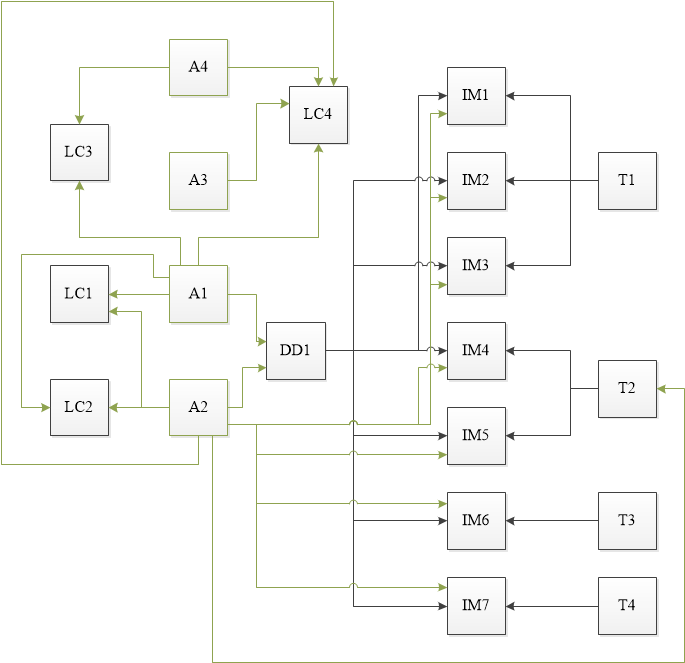
\includegraphics[width=\textwidth]{ATrace.png}
% 		}
% 		\caption{\label{Fig_ATrace} Traceability Matrix Showing the Connections Between Items of Different Sections}
% 	\end{center}
% \end{figure}


% \begin{figure}[h!]
% 	\begin{center}
% 		%\rotatebox{-90}
% 		{
% 			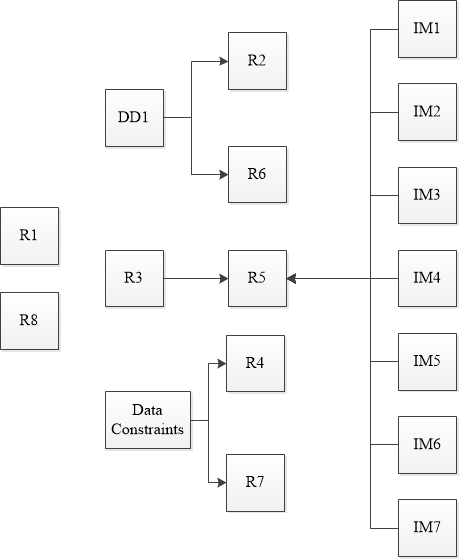
\includegraphics[width=0.7\textwidth]{RTrace.png}
% 		}
% 		\caption{\label{Fig_RTrace} Traceability Matrix Showing the Connections Between Requirements, Instance Models, and Data Constraints}
% 	\end{center}
% \end{figure}

\newpage

\bibliographystyle {plainnat}
\bibliography 
{../../ReferenceMaterial/SRS_Refs,../../ReferenceMaterial/ProblemStatement_Refs}

\newpage

\section{Appendix}

\wss{Your report may require an appendix.  For instance, this is a good point to
show the values of the symbolic parameters introduced in the report.}

\subsection{Symbolic Parameters}

\renewcommand{\arraystretch}{1.2}
\begin{tabular}{l l} 		
	$\varmathbb{R}$ & Domain of real numbers\\
\end{tabular}\\

\end{document}